\documentclass[12pt]{beamer}
%\documentclass[20pt,handout]{beamer}
\usetheme{Frankfurt}
\usepackage{graphicx}
\usepackage{verbatim}
\usepackage[german]{babel}
\usepackage[T1]{fontenc}
\usepackage[utf8]{inputenc}
\setbeamertemplate{footline}[frame number]
\usepackage{multicol}

\usepackage{tikz}
\usetikzlibrary{positioning,arrows}
\tikzstyle{user} = [rectangle, rounded corners, fill=gray!20, bottom color=gray!15, minimum width=50pt]
\tikzstyle{server} = [rectangle, fill=gray!60, bottom color=gray!50, minimum width=60pt, minimum height= 20pt]
\tikzstyle{every path} = [line width=0.4mm]
\tikzstyle{inactive} = [color=gray!30]

% fix appendix

\usepackage{etoolbox}
\makeatletter
\patchcmd{\beamer@part}{\setcounter{subsection}{0}}{}{}
\makeatother

% code listing stuff

\makeatletter
\newcommand{\miniscule}{\@setfontsize\miniscule{5}{6}}% \tiny: 6/7
\makeatother

\usepackage{listings}
\usepackage{color}
\definecolor{lightgray}{rgb}{.9,.9,.9}
\definecolor{darkgray}{rgb}{.4,.4,.4}
\definecolor{purple}{rgb}{0.65, 0.12, 0.82}

\lstdefinelanguage{JavaScript}{
  keywords={typeof, new, true, false, catch, function, return, null, catch, switch, var, if, in, while, do, else, case, break},
  keywordstyle=\color{blue}\bfseries,
  ndkeywords={class, export, boolean, throw, implements, import, this},
  ndkeywordstyle=\color{darkgray}\bfseries,
  identifierstyle=\color{black},
  sensitive=false,
  comment=[l]{//},
  morecomment=[s]{/*}{*/},
  commentstyle=\color{purple}\ttfamily,
  stringstyle=\color{red}\ttfamily,
  morestring=[b]',
  morestring=[b]"
}

\lstset{
   language=JavaScript,
   frame=single,
   backgroundcolor=\color{lightgray},
   extendedchars=true,
   basicstyle=\tiny\ttfamily,
   showstringspaces=false,
   showspaces=false,
   numbers=left,
   numberstyle=\tiny,
   numbersep=9pt,
   tabsize=2,
   breaklines=true,
   showtabs=false,
   captionpos=b
}



\title{\huge WebRTC Security \\ \small Was ist WebRTC und (wieso) ist es sicher?}
\author{Stephan Thamm \\ Innovailable UG \\ www.innovailable.eu}
\date{24.10.2015}

\begin{document}
\maketitle

\frame{\tableofcontents[sections={1-4}]}


\section{Was ist WebRTC?}
\subsection{} 

\begin{frame}
  \frametitle{Was ist WebRTC?}
  \begin{itemize}
    \item<2-> \textbf{Web} \textbf{R}eal \textbf{T}ime \textbf{C}ommunication
    \item<3-> getUserMedia()
    \item<4-> PeerConnection
    \item<5-> DataChannel
  \end{itemize}
\end{frame}

\begin{frame}
  \frametitle{Standardisierung}
  \begin{itemize}
    \item<2-> 2011 von Google initiiert
    \item<3-> WebRTC Gruppe in W3C
    \item<4-> RTCWEB Gruppe in IETF
    \item<5-> Work in Progress
  \end{itemize}
\end{frame}

\begin{frame}
  \frametitle{Implementierung in Browsern}
  \pause
  \centerline{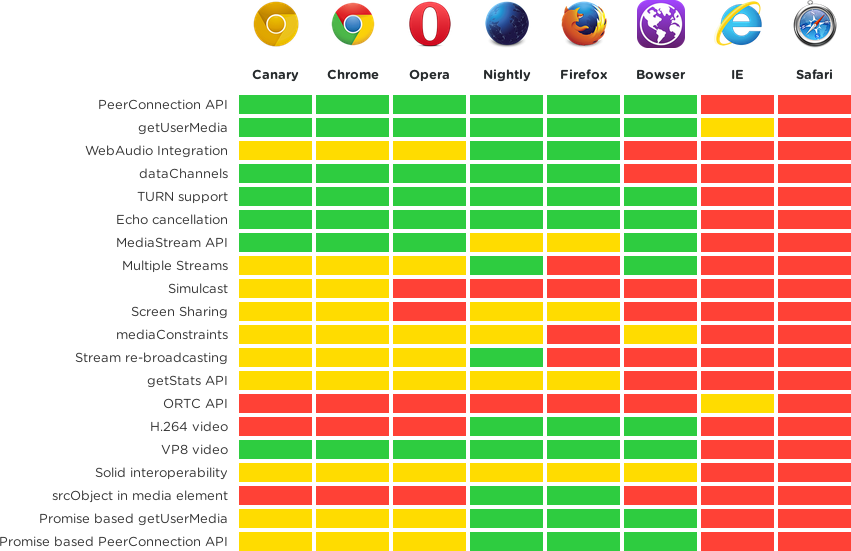
\includegraphics[height=0.7\textheight]{img/webrtc_ready.png}}
  \hfill \tiny http://iswebrtcreadyyet.com/ \\
  \hfill \tiny Stand 23.10.2015
\end{frame}

\begin{frame}
  \frametitle{Palava}
  \includegraphics<1>[height=0.7\textheight]{img/palava_1.jpg}
  \includegraphics<2>[height=0.7\textheight]{img/palava_2.jpg}
  \includegraphics<3>[height=0.7\textheight]{img/palava_3.jpg}
  \\ \hfill \tiny https://palava.tv
\end{frame}

\begin{frame}
  \frametitle{Sharefest}
  \centerline{
\includegraphics[width=0.5\textwidth]{img/sharefest.png}}
  \centerline{\tiny https://sharefest.me}
\end{frame}

\begin{frame}
  \frametitle{Cube Slam}
  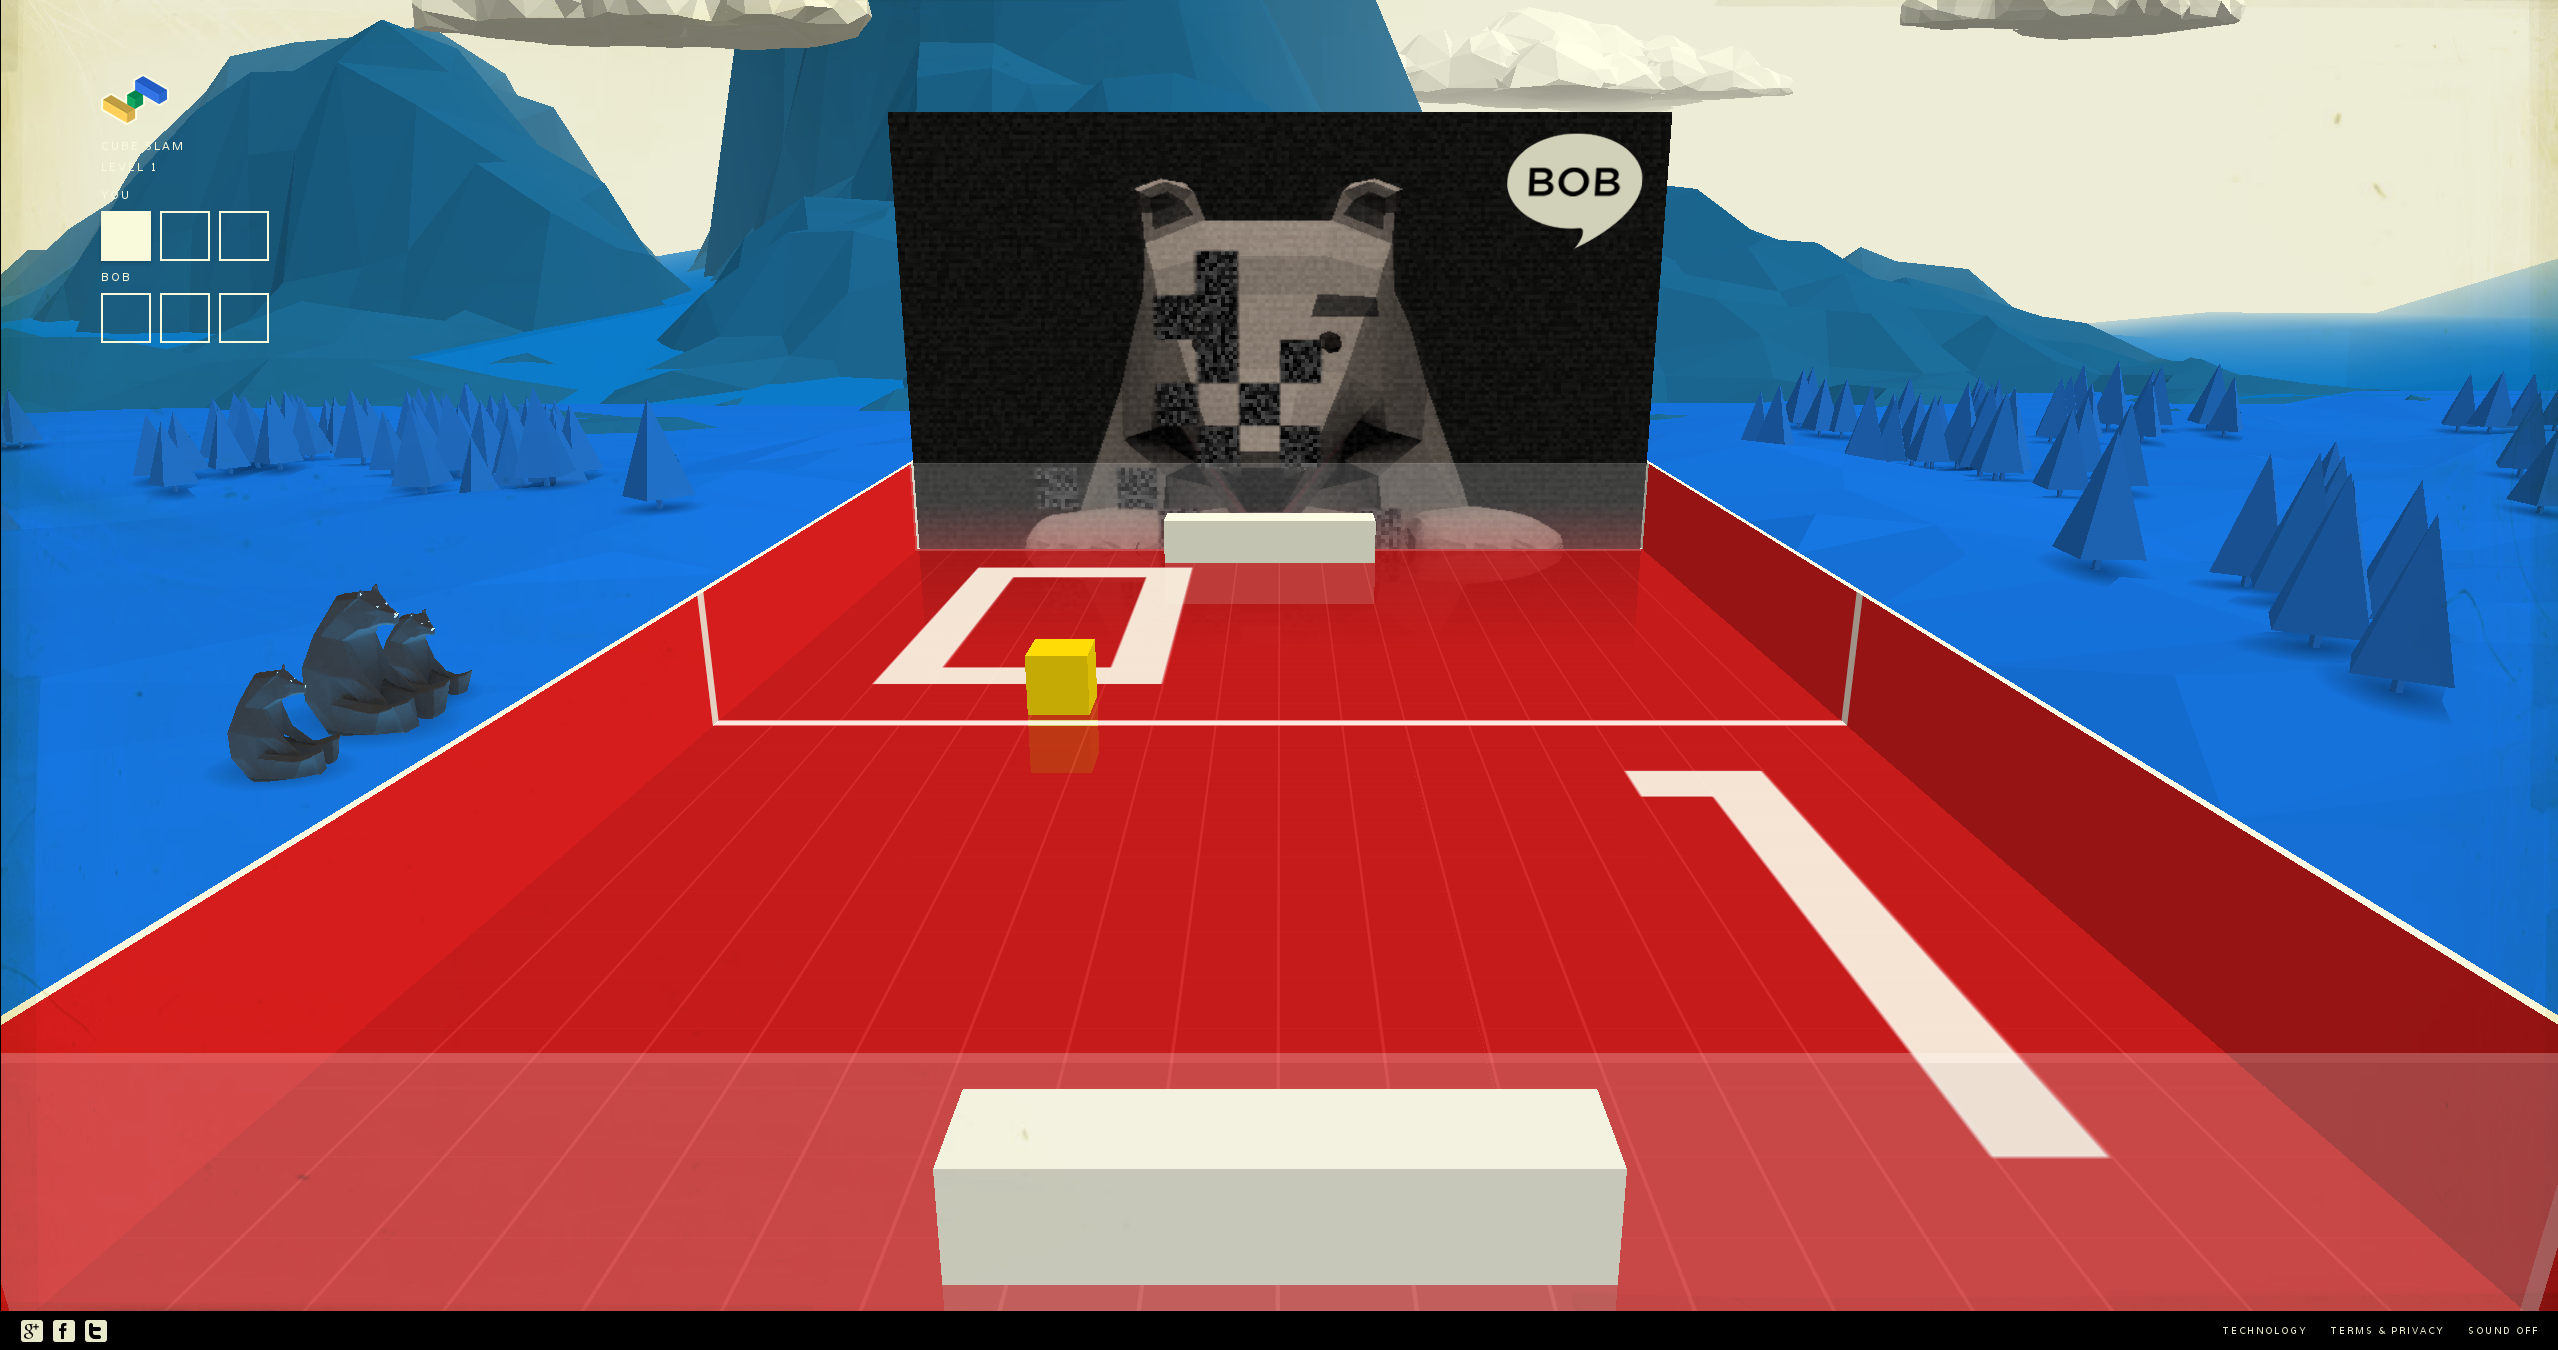
\includegraphics[height=0.7\textheight]{img/cube_slam.png} \\
  \hfill \tiny https://www.cubeslam.com
\end{frame}

\begin{frame}
  \frametitle{BananaBread}
  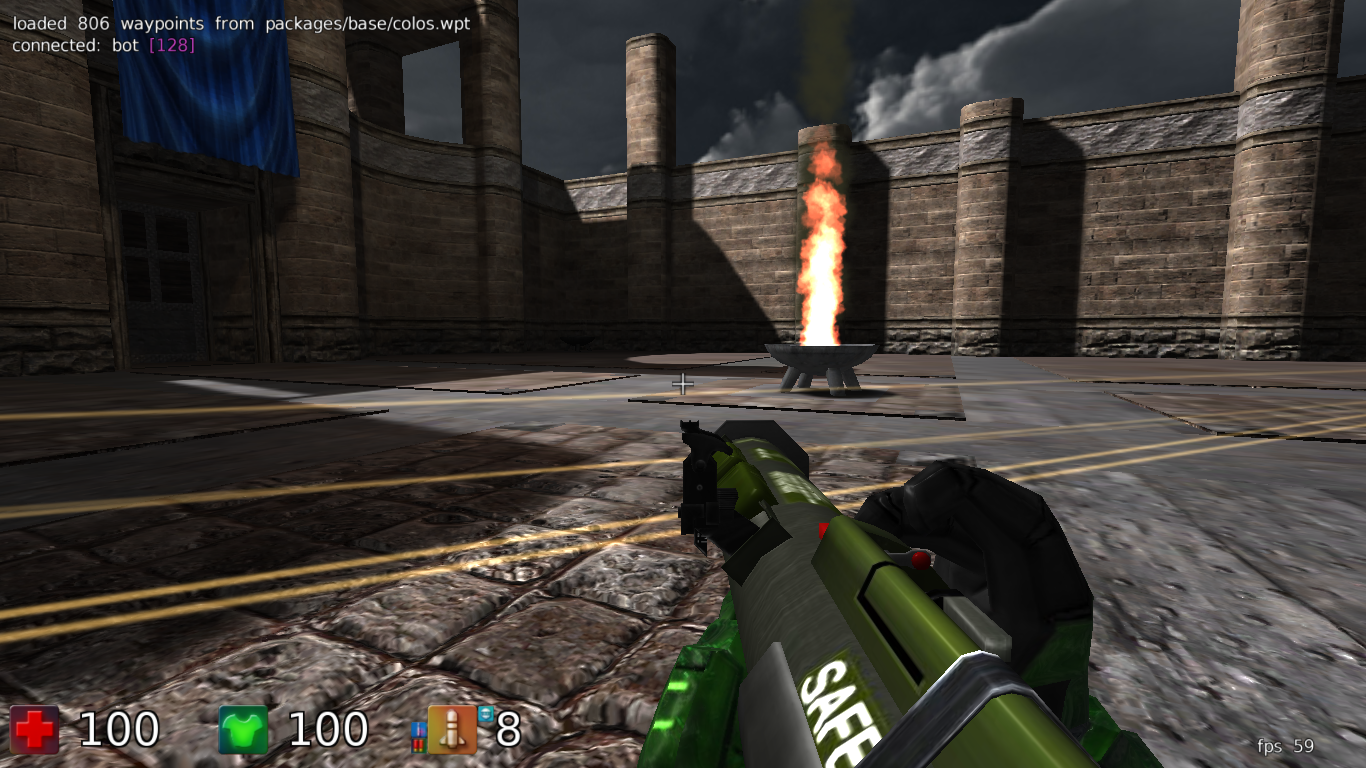
\includegraphics[height=0.7\textheight]{img/bananabread.png} \\
  \hfill \tiny https://developer.mozilla.org/de/demos/detail/bananabread
\end{frame}

\begin{frame}
  \frametitle{Verbreitung}
  \begin{center}
    \pause
    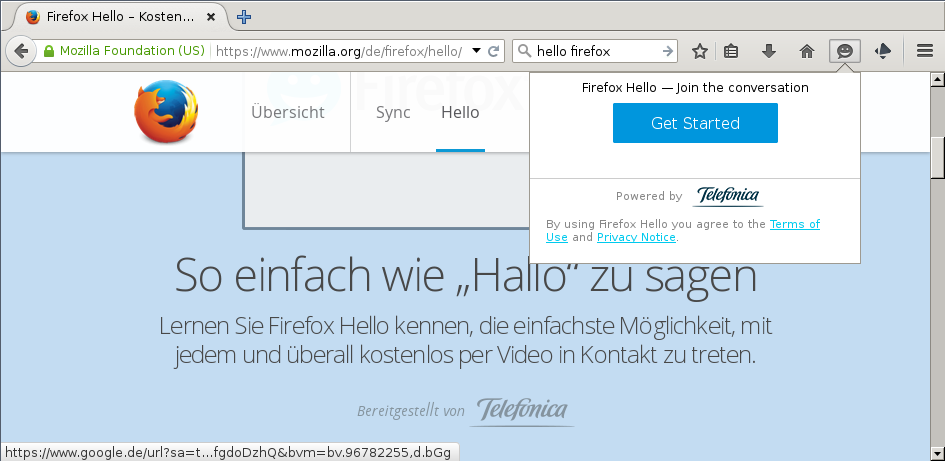
\includegraphics[height=0.4\textheight]{img/hello_firefox.png} \\
    \pause
    
\includegraphics[height=0.3\textheight]{img/facebook.jpg}
  \end{center}
\end{frame}


\section{Anwendungssicht}
\subsection{} 

\begin{frame}
  \frametitle{getUserMedia()}
  \pause
  \lstinputlisting[basicstyle=\footnotesize\ttfamily,numberstyle=\footnotesize]{examples/gum.js}
\end{frame}

\begin{frame}
  \frametitle{Kamerazugriff}
  \pause
  \centerline{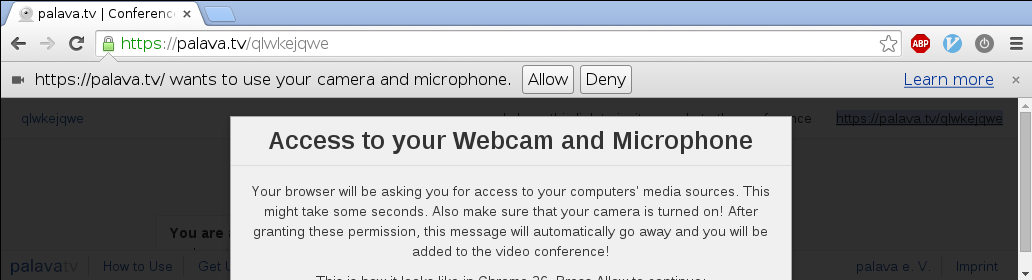
\includegraphics[width=0.7\textwidth]{img/access_chrome.png}}
  %\hfill \tiny Chrome
  \vspace{15pt}
  \centerline{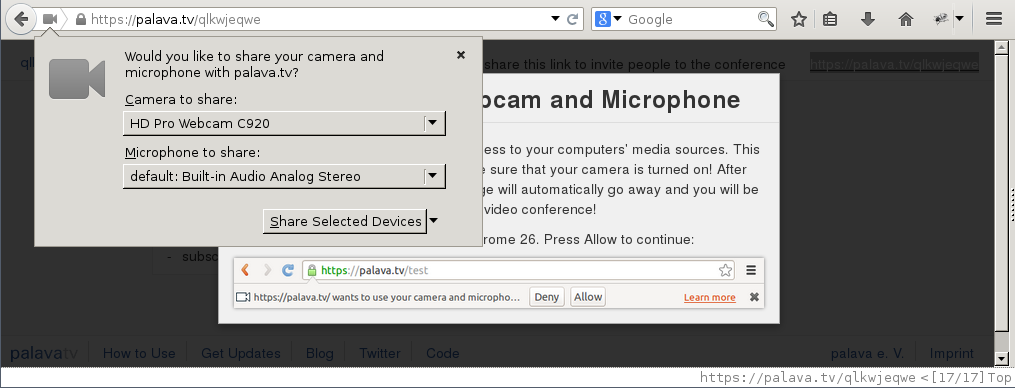
\includegraphics[width=0.7\textwidth]{img/access_firefox.png}}
  %\hfill \tiny Firefox
\end{frame}

\begin{frame}
  \frametitle{Peer to Peer}
  \pause
  \centerline{\begin{tikzpicture}[transform shape]
  \tikzstyle{every node} = [user]

  \onslide<+-> {
    \node (a) at (180: 4) {Alice};
  }

  \onslide<+-> {
    \node (b) at +(0: 4) {Bob};
  }

  \onslide<+-> {
    \draw [<->] (a) -- (b);
  }

  \onslide<+->{
    \node (c) at +(90: 2) {Charlie};
  }

  \onslide<+->{
    \draw [<->] (a) -- (c);
  }

  \onslide<+->{
    \draw [<->] (b) -- (c);
  }

  \onslide<+->{
    \node (d) at +(270: 2) {Dave};
  }

  \onslide<+->{
    \foreach \from/\to in {a/d, b/d, c/d}
      \draw [<->] (\from) -- (\to);
  }
\end{tikzpicture}
}
\end{frame}

\begin{frame}
  \frametitle{Multipoint Control Unit (MCU)}
  \pause
  \centerline{\begin{tikzpicture}[transform shape]
  \onslide<+->{
    \node[server, minimum width=80pt, minimum height= 30pt] (mcu) at (0, 0) {\large MCU};
  }

  \onslide<+->{
    \node[user] (a) at (150: 4) {Alice};
    \node[user] (b) at +(30: 4) {Bob};
    \node[user] (c) at +(210: 4) {Charlie};
    \node[user] (d) at +(330: 4) {Dave};
  }

  \onslide<+->{
    \foreach \from/\to in {a/mcu, b/mcu, c/mcu, d/mcu}
      \draw [<->] (\from) -- (\to);
  }
\end{tikzpicture}
}
\end{frame}


\section{Verbindungsaufgbau}
\subsection{} 

\begin{frame}
  \frametitle{Ablauf Verbindungsaufgbau}
  \centerline{\begin{tikzpicture}[transform shape]
  \onslide<+>{}

  % alice and bob introduction

  \onslide<+->{
    \node[user] (a) at (2, 0) {Alice};
    \node[user] (b) at (6, 0) {Bob};
  }

  % how to peer connection?

  \onslide<+>{
    \node (offer) at (4, 0.8) {PeerConnection};
    \draw [dotted, <->] (a) -- (b);
  }

  \onslide<+>{}

  % download webapp

  \onslide<6-7>{
    \node (offer) at (4, 2) {Download Webapp};
  }

  \onslide<+->{
    \node[server] (web) at (0, 3) {\large Webserver};
  }

  \onslide<+>{
    \draw [->] (web) -- (a);
  }

  \onslide<+>{
    \draw [inactive, ->] (web) -- (a);
    \draw [->] (web) -- (b);
  }

  \onslide<+>{}

  % signaling

  \onslide<+->{
    \node[server] (signaling) at (4, 3) {\large Signaling};
  }

  % offer

  \onslide<10-11>{
    \node (offer) at (4, 1) {Offer};
  }

  \onslide<+>{
    \draw [->] (a) -- (signaling);
  }

  \onslide<+>{
    \draw [inactive, ->] (a) -- (signaling);
    \draw [->] (signaling) -- (b);
  }

  \onslide<+>{}

  % answer

  \onslide<13-14>{
    \node (offer) at (4, 1) {Answer};
  }
  \onslide<+>{
    \draw [->] (b) -- (signaling);
  }

  \onslide<+>{
    \draw [inactive, ->] (b) -- (signaling);
    \draw [->] (signaling) -- (a);
  }

  \onslide<+>{}

  % stun

  \onslide<+->{
    \node[server] (stun) at (8, 3) {\large STUN};
  }

  % ice b

  \onslide<17-18>{
    \node (offer) at (6, 2.3) {Hole Punching};
  }

  \onslide<+>{
    \draw [<->] (b) -- (stun);
  }

  \onslide<+>{
    \draw [inactive, <->] (b) -- (stun);
    \draw [->] (b) -- (signaling);
    \draw [->] (signaling) -- (a);
  }

  \onslide<+>{}

  % ice a

  \onslide<20-21>{
    \node (offer) at (7, 1.2) {Hole Punching};
  }

  \onslide<+>{
    \draw [<->] (a) -- (stun);
  }

  \onslide<+>{
    \draw [inactive, <->] (a) -- (stun);
    \draw [->] (a) -- (signaling);
    \draw [->] (signaling) -- (b);
  }

  \onslide<+>{}

  % peer connection done

  \onslide<+>{
    \node (offer) at (4, 0.8) {PeerConnection};
    \draw [<->] (a) -- (b);
  }

\end{tikzpicture}
}
\end{frame}

\begin{frame}
  \frametitle{Session Description Protocol (SDP)}
  \pause
  \begin{multicols}{2}
    \lstinputlisting[language={},numbers=none,basicstyle=\miniscule\ttfamily]{examples/sdp.txt}
  \end{multicols}
\end{frame}

\begin{frame}
  \frametitle{m Lines}

  \only<2>{
    \lstinputlisting[language={},firstline=8,lastline=24]{examples/sdp.txt}
    \hfill \tiny Auszug Offer/Answer
  }

  \only<3>{
    \lstinputlisting[language={},firstline=25,lastline=36]{examples/sdp.txt}
    \hfill \tiny Auszug Offer/Answer
  }

  \only<4>{
    \lstinputlisting[language={},firstline=37,lastline=42]{examples/sdp.txt}
    \hfill \tiny Auszug Offer/Answer
  }
\end{frame}

\begin{frame}
  \frametitle{Interactive Connectivity Establishment (ICE)}
  \pause
  \lstinputlisting[language={},numbers=none,firstline=34,lastline=35,basicstyle=\tiny\ttfamily]{examples/sdp.txt}
  \hfill \tiny Auszug Offer/Answer
  \vspace{15pt}
  \pause
  \lstinputlisting[language={},numbers=none,basicstyle=\tiny\ttfamily,firstline=1,lastline=1]{examples/ice_trickle.txt}
  \lstinputlisting[language={},numbers=none,basicstyle=\tiny\ttfamily,firstline=2,lastline=2]{examples/ice_trickle.txt}
  \hfill \tiny ICE Trickling
\end{frame}


\section{Bibliotheken}
\subsection{} 

\begin{frame}
  \frametitle{palava-client}
  \pause
  \lstinputlisting[basicstyle=\tiny\ttfamily,numberstyle=\tiny]{examples/palava.js}
  \hfill \tiny https://github.com/palavatv/palava-client
\end{frame}

\begin{frame}
  \frametitle{rtc-lib}
  \pause
  \lstinputlisting[basicstyle=\tiny\ttfamily,numberstyle=\tiny]{examples/rtc-lib.js}
  \hfill \tiny https://github.com/Innovailable/rtc-lib
\end{frame}

\begin{frame}
  \frametitle{easy-signaling}
  \pause
  \lstinputlisting[basicstyle=\tiny\ttfamily,numberstyle=\tiny]{examples/easy-signaling.js}
  \hfill \tiny https://github.com/Innovailable/easy-signaling
\end{frame}


\section{Fazit}
\subsection{}

\begin{frame}
  \frametitle{Was brauche ich für WebRTC?}
  \begin{itemize}
    \onslide<+->{}
    \item<+-> eine passende Idee
    \item<+-> WebRTC Bibliothek
    \begin{itemize}
      \item<+-> rtc-lib \onslide<+->{, palava-client} \onslide<+->{, native} \onslide<+->{\dots}
    \end{itemize}
    \item<+-> Signaling Server
    \begin{itemize}
      \item<+-> easy-signaling\onslide<+->{, palava-machine}\onslide<+->{ \dots}
      \item<+-> wss://rtc.innovailable.eu/ (rtc-lib)
      \item<+-> wss://signaling.innovailable.eu/ (palava-client)
    \end{itemize}
    \item<+-> STUN-Server\onslide<+->{ + evtl TURN-Server}
    \begin{itemize}
      \item<+-> stun\onslide<+->{, coturn}\onslide<+->{ \dots}
    \end{itemize}
    \item<+-> klassische Webentwicklung
  \end{itemize}
\end{frame}

\begin{frame}
  \frametitle{Fragen? Antworten!}

  \centerline{\scriptsize{Kontakt}}
  \centerline{stephan@innovailable.eu}
  \centerline{www.innovailable.eu}
  \centerline{@chaossource}

  \vspace{0.2in}

  \centerline{\scriptsize{Slides}}
  \centerline{https://github.com/Innovailable/webrtc-security-talk}
\end{frame}

\end{document}
